% -*-latex-*-

\chapter{Physics Motivation}
\label{C4}

In previous chapters, we have discussed the unpolarized and polarized structure functions and their relations to the parton model. These structure functions have been extracted over a wide kinematic range during the past 40 years. However, data on the spin structure function $g_2$ at low energy are still lacking. Jefferson Lab Experiment E08-027 will provide precise $g_2$ data for the proton in the resonance region and extract the generalized longitudinal-transverse polarizability $\dlt$. $\dlt$ is expected to be a good test for the Chiral Perturbation Theory, as mentioned in \Cref{C3S1}. In addition, the $g_2$ data in the low $Q^2$ region could be used to provide a test of the Burkhardt-Cottingham (BC) sum rule. In this chapter, we will first give an overview of previous experiments of structure function measurements. The generalized longitudinal-transverse polarizability $\dlt$ and the BC sum rule will be discussed as the major motivation of E08-027. The low $Q^2$ $g_2$ data will also help to improve the precision of the hyperfine structure calculation of hydrogen, which will also be discussed in this chapter.

\section{\texorpdfstring{Existing $g_2$ Data}{Existing g2 Data}}
\label{C4S1}

In \Cref{C2S2}, the relations between the spin structure functions and the cross-sections have been given as \cref{C2S2E25,C2S2E26}. To extract the spin structure functions $g_1$ and $g_2$, one natural way is to measure the cross-section differences, which are defined as:
\begin{align} \label{C4S1E1}
\Delta\sigma_{\parallel} & = \dd{\sigma}^{\buildrel\rightarrow\over\Leftarrow}-\dd{\sigma}^{\buildrel\rightarrow\over\Rightarrow}, \\ \label{C4S1E2}
\Delta\sigma_{\perp} & = \dd{\sigma}^{\rightarrow\Uparrow}-\dd{\sigma}^{\rightarrow\Downarrow},
\end{align}
where the single arrow and the double arrow indicate the polarization of the electrons and the target respectively: $\buildrel\rightarrow\over\Leftarrow$ and $\buildrel\rightarrow\over\Rightarrow$ means the target is longitudinal polarized, $\rightarrow\Uparrow$ and $\rightarrow\Downarrow$ means the target is transversely polarized. The second method is to measure the asymmetries which typically have reduced systematic uncertainty. The longitudinal asymmetry $A_{\parallel}$ and transverse asymmetry $A_{\perp}$ can be defined straightforwardly:
\begin{align} \label{C4S1E3}
A_{\parallel} & = \frac{\dd{\sigma}^{\buildrel\rightarrow\over\Leftarrow}-\dd{\sigma}^{\buildrel\rightarrow\over\Rightarrow}}{\dd{\sigma}^{\buildrel\rightarrow\over\Leftarrow}+\dd{\sigma}^{\buildrel\rightarrow\over\Rightarrow}} = \frac{\Delta\sigma_{\parallel}}{2\dd{\sigma}_{\mathrm{unpol}}}, \\ \label{C4S1E4}
A_{\perp} & = \frac{\dd{\sigma}^{\rightarrow\Uparrow}-\dd{\sigma}^{\rightarrow\Downarrow}}{\dd{\sigma}^{\rightarrow\Uparrow}+\dd{\sigma}^{\rightarrow\Downarrow}} = \frac{\Delta\sigma_{\perp}}{2\dd{\sigma}_{\mathrm{unpol}}}.
\end{align}
From the photon-absorption cross-sections formulation discussed in \Cref{C2S4SS1}, we could define two more asymmetries via \cref{C2S4SS1E6,C2S4SS1E7,C2S4SS1E8,C2S4SS1E9}:
\begin{align} \label{C4S1E5}
A_1 & = \frac{\stt}{\sigma_{T}} = \frac{g_1-\gamma^2g_2}{F_1}, \\ \label{C4S1E6}
A_2 & = \frac{\slt}{\sigma_{T}} = \frac{\gamma(g_1+g_2)}{F_1},
\end{align}
where $\gamma=Q/\nu$.

One can measure the longitudinal and transverse cross-section differences $\sigma_\parallel$ and $\sigma_\perp$ to extract $g_2$. As an alternative way, it is also possible to measure the asymmetries $A_\parallel$, $A_\perp$ or $A_1$, $A_2$ and combine with existing $F_1$ results to extract $g_2$.

SLAC represented the earliest results for $g_2$ structure function in the DIS region \cite{Anthony1996}. During the same time, the SMC group at CERN used deep inelastic muon-nucleon scattering to extract the $g_1$ and $g_2$ structure functions for a proton target \cite{Adams1997}. Since $g_2$ is relatively small, more statistics are always required to extract it than for the extraction of $g_1$. Thus, some of the experiments like the SLAC E155x \cite{Anthony2003} focused on transversely polarized targets to achieve enough statistics and extracted $g_2$ using existing $g_1$ or $A_1$ data. The most recent results came from Jefferson Lab, where several experiments have collected a large amount of data covering a wide $Q^2$ range with a high intensity polarized electron beam. These JLab measurements covered both DIS and resonance regions.

\begin{figure}[b!]
  \centering
  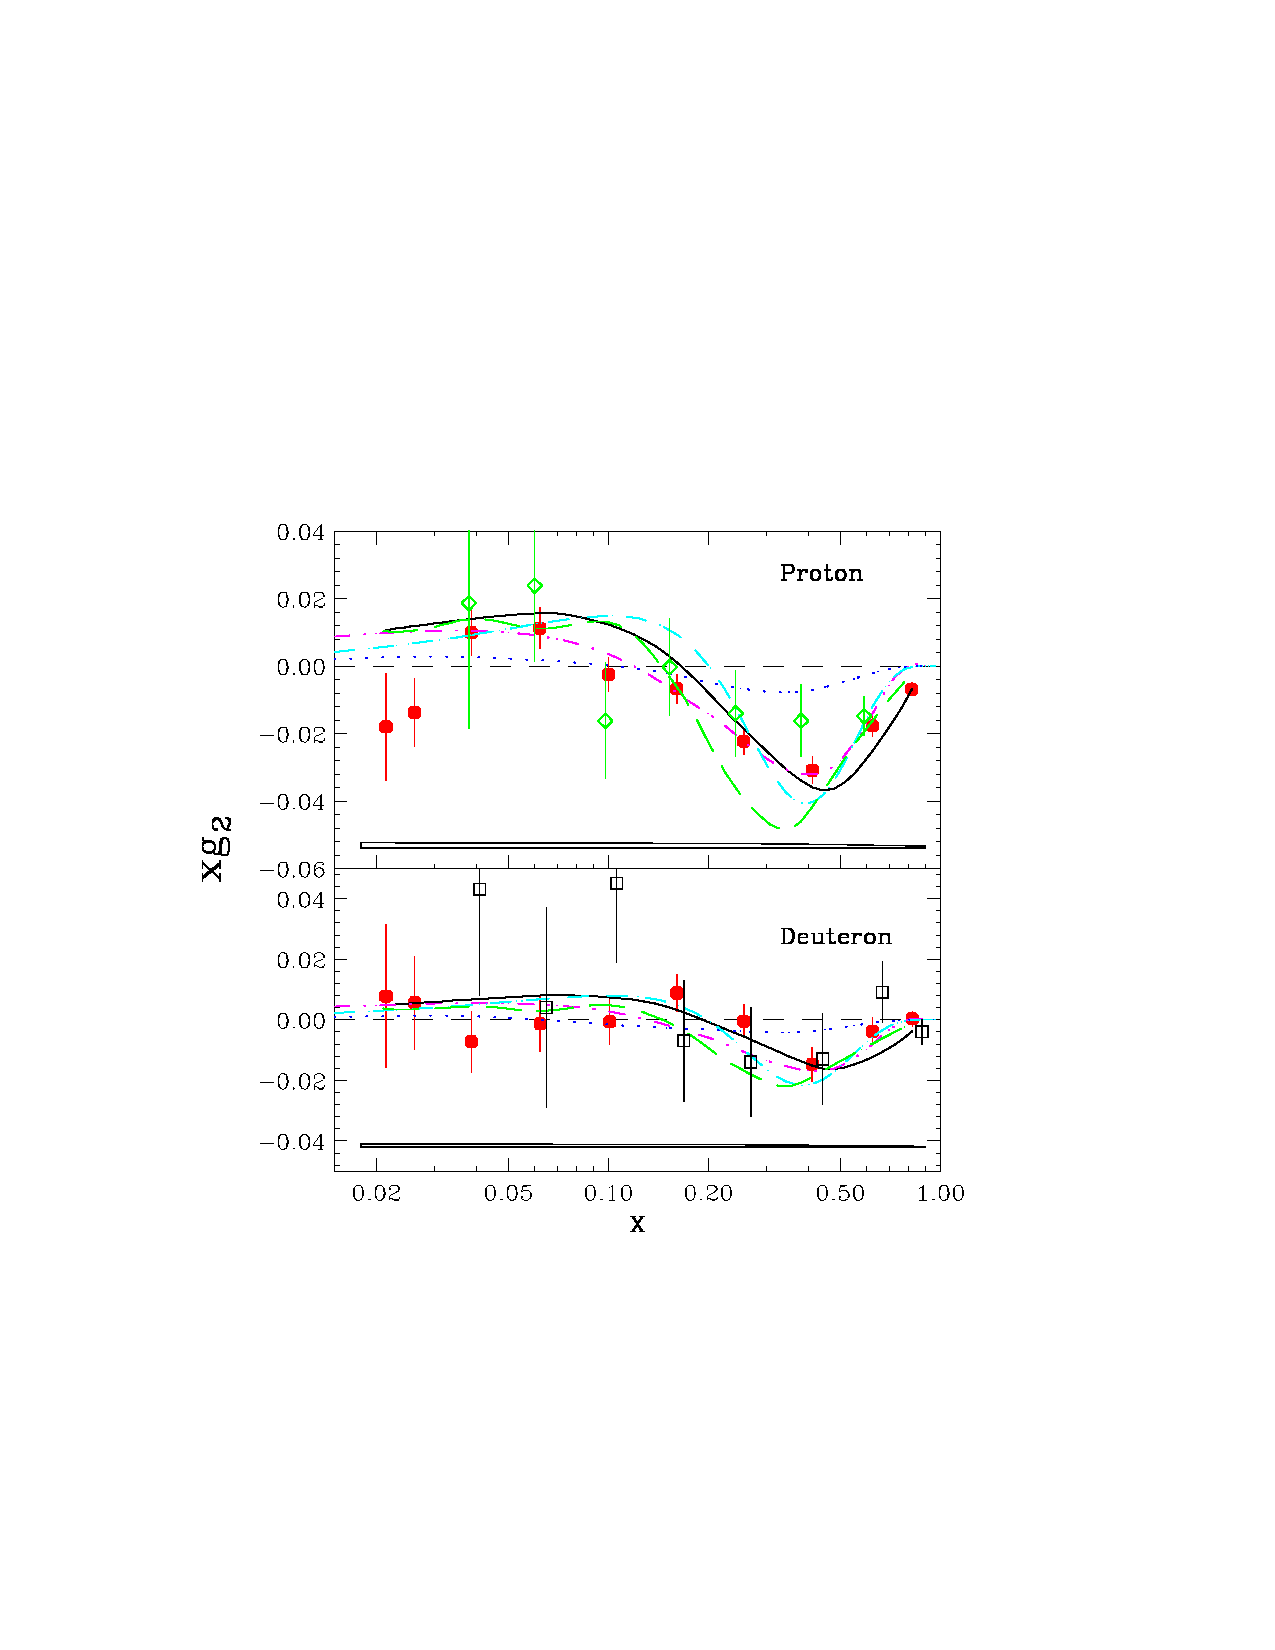
\includegraphics[width=0.75\textwidth]{figs/xg2p_E155x.pdf}
  \caption[$xg_2$ data from SLAC E155x, E143 and E155.]{$xg_2$ data from E155x \cite{Anthony2003} (solid circle), E143 \cite{Abe1998} (open diamond) and E155 \cite{Anthony2003} (open square). The $\gtww$ calculation result at the average $Q^2$ of E155x is also shown as the solid line as well as some model estimations from Stratmann \cite{Stratmann1993} (dash-dot), Song \cite{Song1996} (dot), Weigel and Gamberg \cite{Weigel2001} (short dash) and Wakamatsu \cite{Wakamatsu2000} (long dash). Plot reproduced from \cite{Anthony2003}. \label{C4S1F1}}
\end{figure}

The most precise DIS measurement results of $g_2$ for proton and deuteron targets were represented by SLAC E155x \cite{Anthony2003}. The kinematic range was $0.02\leq x\leq 0.8$ and $0.7\leq Q^2 \leq 20$ GeV${}^2$. The SLAC E143 \cite{Abe1998} and E155 \cite{Anthony2003} also contributed to the $g_2$ measurement of proton. The $g_2$ results from SLAC E143, E155 and E155x are shown in \Cref{C4S1F1}. The solid curve in the figure represents the $\gtww$ calculation results using $g_1$ data. The curve shows that the measurement and the leading twist estimation are consistent. However, the large error bars do not exclude the possible higher-twist effects.

As mentioned above, JLab also measured the $g_2$ structure function in the DIS region. The JLab E97-103 measured $g_2$ for neutrons and reported a two standard deviation difference from the leading twist expectation of $g_2^n$ \cite{Kramer2005}. The $Q^2$ coverage of this experiment is $0.58<Q^2<1.36$ GeV${}^2$ at $x\approx0.2$. \Cref{C4S1F2} shows the $xg_2^n$ results from JLab E97-103 \cite{Kramer2005}, E99-117 \cite{Zheng2004} and SLAC E155 \cite{Anthony2003}. The figure clearly represents the deviation between the experimental results and the leading twist estimation.

\begin{figure}[tb!]
  \centering
  \setlength{\unitlength}{0.1\textwidth}
  \begin{picture}(6.5,4.2)
    \put(0,0){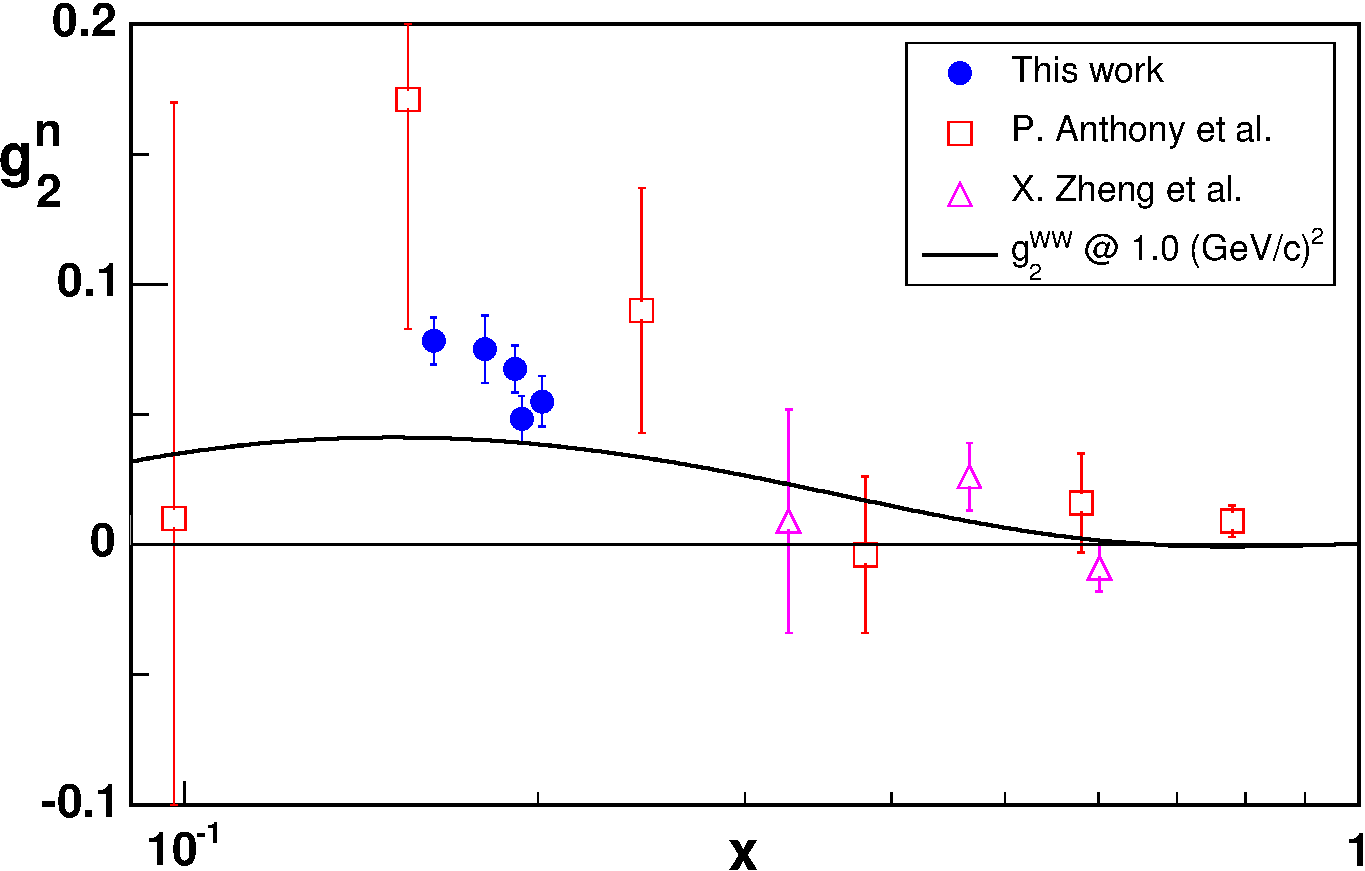
\includegraphics[width=0.65\textwidth]{figs/xg2n_E97103.pdf}}
    \put(4.2,2.8){\colorbox{white}{\makebox(2.1,1.1){\textcolor{white}{a}}}}
  \end{picture}
  \caption[$xg_2^n$ data from E97-103.]{$xg_2^n$ data from E97-103 \cite{Kramer2005} (solid circle), E99-117 \cite{Zheng2004} (open triangle) and E155 \cite{Anthony2003} (open square). The solid curve shows $\gtww$ calculation at $Q^2=1.0$ GeV${}^2$. Plot reproduced from \cite{Kramer2005}. \label{C4S1F2}}
\end{figure}

From the discussion in \Cref{C3S1SS3}, we know that the quark-gluon interaction has a stronger effect in the resonance region. The first experiment to measure $g_2$ in the resonance region was the SLAC E143, at $Q^2=0.5$ GeV${}^2$ and 1.2 GeV${}^2$ \cite{Abe1998}. However the error bars were large for this measurement. JLab E94-010 collected a large amount of data to extract the neutron $g_2$ structure function at low $Q^2$ \cite{Amarian2004a}. The structure function $g_2$ was extracted from the longitudinal and transverse cross-section differences of a polarized ${}^3$He target. The results of ${}^3$He $g_2$ are shown in \Cref{C4S1F3}, which shows a significant deviation from the $\gtww$ estimation.

\begin{figure}[p!]
  \centering
  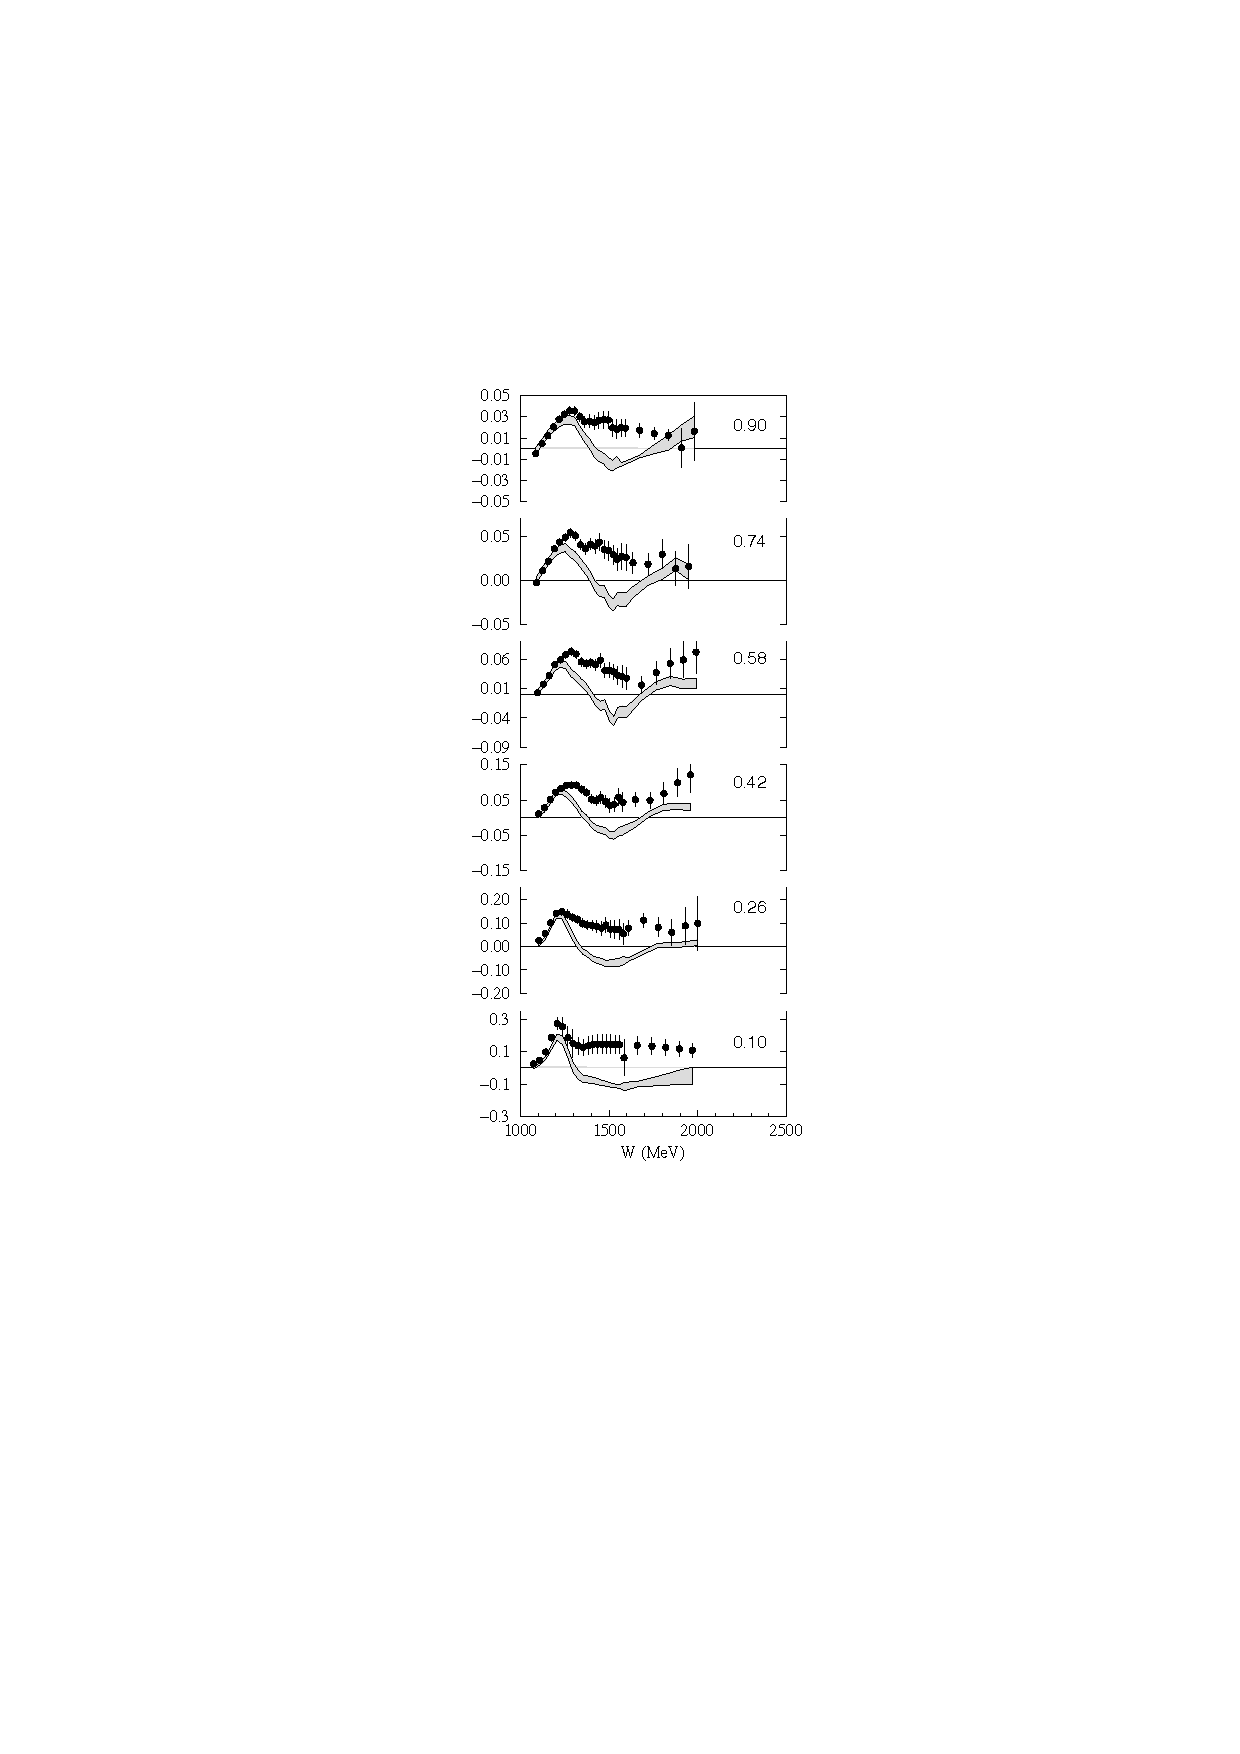
\includegraphics[width=0.55\textwidth]{figs/g2_E94010.pdf}
  \caption[${}^3$He $g_2$ data from E94-010.]{${}^3$He $g_2$ data from E94-010. The constant $Q^2$ values are indicated in GeV${}^2$ in each panel. The grey bands represent the $\gtww$ expectations at each corresponding $Q^2$ value. Plot reproduced from \cite{Amarian2004a}. \label{C4S1F3}}
\end{figure}

The Resonance Spin Structure (RSS) collaboration in JLab Hall B measured the proton $g_2$ structure function at $Q^2=1.3$ GeV${}^2$ \cite{Wesselmann2007}. Currently this is the lowest $Q^2$ measurement of $g_2^p$. The results are shown in \Cref{C4S1F4}. The leading twist behavior is clearly insufficient to describe the data.

\begin{figure}[tb!]
  \centering
  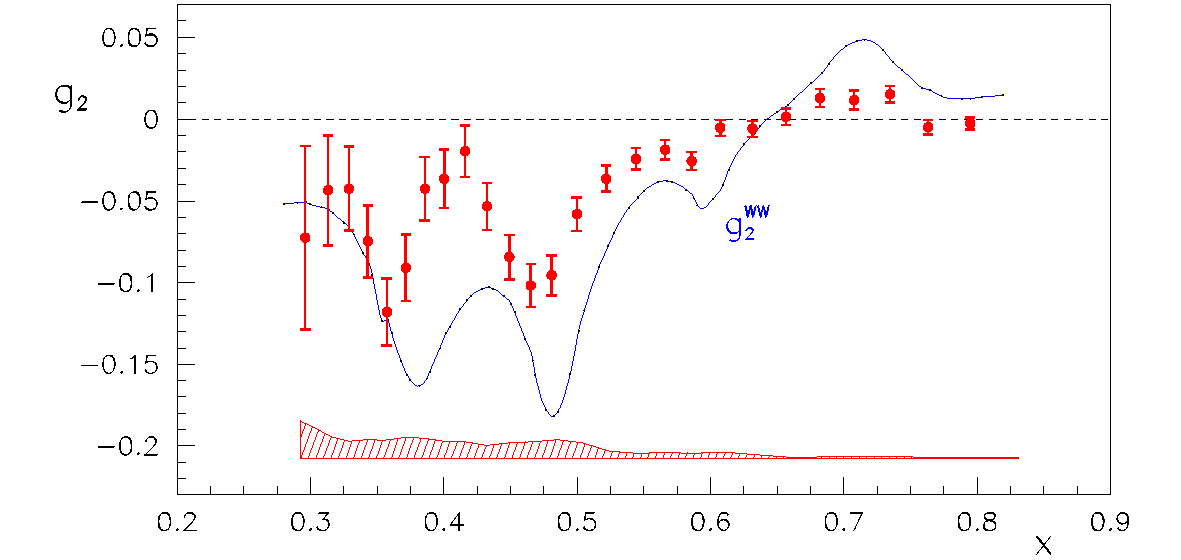
\includegraphics[width=0.9\textwidth]{figs/g2_RSS.pdf}
  \caption[Proton $g_2$ data from RSS experiment.]{Proton $g_2$ data from RSS experiment compared with the $\gtww$ expectations at $Q^2=1.3$ GeV${}^2$. Plot reproduced from \cite{Wesselmann2007}. \label{C4S1F4}}
\end{figure}

\section{Existing Data for Spin Polarizabilities}
\label{C4S2}

From the discussion in \Cref{C2S4}, we know that the nucleon polarizabilities are fundamental observables that characterize nucleon structure. The electric and magnetic polarizabilities $\alpha$ and $\beta$ describe the response of a nucleon to an external electromagnetic field. Real photon Compton scattering experiments were performed to measure these two quantities since they are related to the spin non-flip forward Compton scattering amplitude \cite{Olmos2001,Tonnison1998}. The forward spin polarizability $\gamma_0$ is associated with the spin flip amplitude. It has been measured at MAMI (Mainz) with a circularly polarized photon beam on a longitudinally polarized proton target \cite{Ahrens2001}.

In the previous section, we have discussed that these polarizabilities could be generalized in VVCS. The generalized polarizabilities defined in \cref{C2S4SS3E8,C2S4SS3E12} have an extra $1/\nu^2$ weighting in the integrand compared to the corresponding leading moments. Thus, the contribution of the large-$\nu$ region to these integrals are suppressed by this weight. With this suppression effect, the generalized spin polarizabilities become a perfect tool to probe the nucleon structure in the chiral perturbation region. The generalized polarizabilities have been evaluated with next-to-leading order (NLO) $\chi$PT calculations at low $Q^2$ \cite{Bernard2003,Kao2003}. As mentioned in \Cref{C3S1SS3}, the nucleon resonances, especially the $\Delta$ resonance, play an important role in the $\chi$PT calculations. Ref. \cite{Bernard2003} and \cite{Kao2003} have pointed out that the generalized longitudinal polarizability $\dlt$ is insensitive to the $\Delta$ resonance compare with the generalized forward spin polarizability $\gamma_0$. The effects from the $\Delta$ resonance contribution are expected to be important in $\gamma_0$ but are supposed to largely cancel in $\dlt$.

\begin{figure}[tb!]
  \centering
  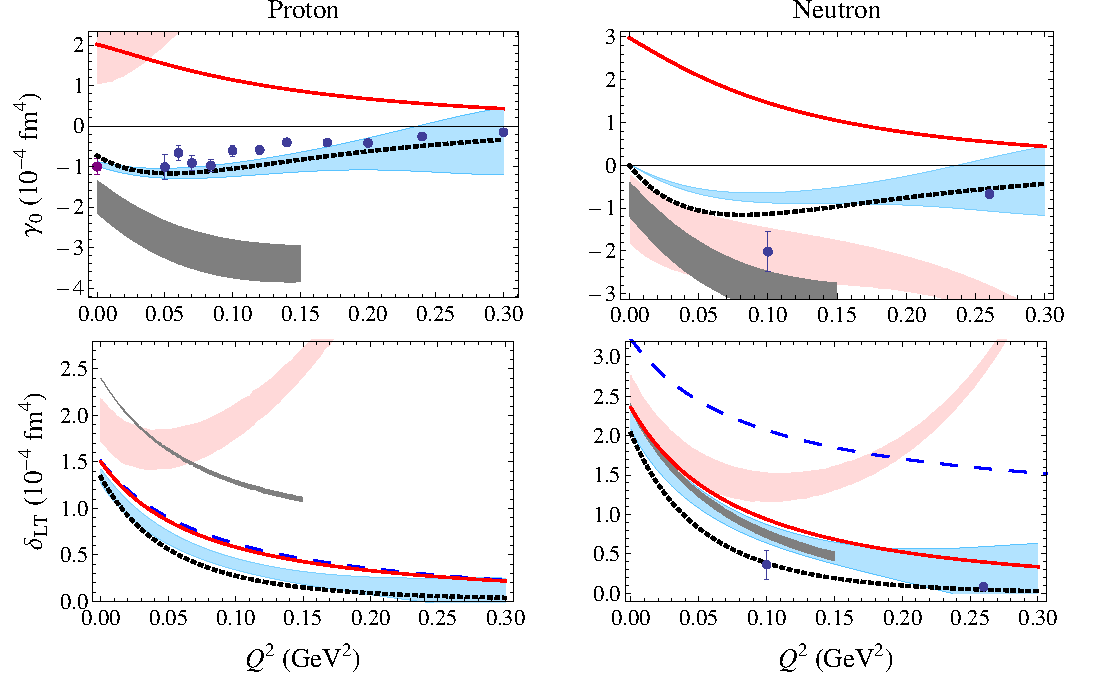
\includegraphics[width=\textwidth]{figs/g0_dlt_xpt.pdf}
  \caption[Generalized spin polarizability $\gamma_0$ and $\dlt$ of proton and neutron.]{Generalized spin polarizability $\gamma_0$ and $\dlt$ of proton and neutron. The neutron data are from E94-010 experiment \cite{Amarian2004b}. The proton data at $Q^2=0$ (purple dot) are from ELSA \cite{Dutz2003}, and at finite $Q^2$ (blue dots) from EG1 experiment at JLab \cite{Prok2009}. The blue dashed line is the HB$\chi$PT calculation \cite{Kao2003}, off the scale in the upper panels. The red bands shows the IR version of RB$\chi$PT calculation \cite{Bernard2003}. The grey bands are the first RB$\chi$PT calculation from Ref. \cite{Bernard2013}. The red solid lines and blue bands shows the most recent LO and NLO RB$\chi$PT calculations respectively \cite{Lensky2014}. Black dotted lines represents the empirical evaluation using the Mainz online partial-wave analysis of meson electroproduction (MAID). Plot reproduced from \cite{Lensky2014}. \label{C4S2F1}}
\end{figure}

The experimental results compared with the $\chi$PT calculations are shown in \Cref{C4S2F1}. The first results of neutron $\gamma_0(Q^2)$ and $\dlt(Q^2)$ were obtained from JLab Hall A E94-010 \cite{Amarian2004b} (blue dots in the neutron panels). The data are compared with a HB$\chi$PT calculation \cite{Kao2003} (blue dashed line) and an infrared-regularized (IR) version of RB$\chi$PT calculation \cite{Bernard2003} (red bands) which is relativisitic but has an unphysical analytic structure. At the lowest $Q^2$ point, the IR version of RB$\chi$PT calculation of $\gamma_0$ including the resonance contributions agrees with the experimental result from E94-010 for neutron. But there are discrepancies between the HB$\chi$PT calculation of $\gamma_0$ and the experimental result even at the lowest $Q^2$ point. For $\dlt$, both the HB$\chi$PT calculation and the IR version of RB$\chi$PT calculation indicates a significant disagreement with the data, which is known as the ``$\dlt$ puzzle''. Since the $\dlt$ is insensitive to the $\Delta$ resonance contribution, it is believed that $\dlt$ is a more suitable testing base for the $\chi$PT compare with $\gamma_0$. A first RB$\chi$PT calculation (with no unphysical analytical structure) from Ref. \cite{Bernard2013} shows that it agrees much better than the HB$\chi$PT and the IR version of the RB$\chi$PT for $\gamma_0$ (grey bands). The most recent calculation from Ref. \cite{Lensky2014} using LO and NLO RB$\chi$PT shows that the $\dlt$ data agrees with their NLO calculation (blue bands). The neutron $\gamma_0$ and $\dlt$ data in \Cref{C4S2F1} is obtained from the JLab E94-010. The proton $\dlt$ data is required to complete the comparison. This is one of the major physics motivation of the JLab E08-027.

\section{Burkhardt-Cottingham Sum Rule}
\label{C4S3}

In \Cref{C2S4SS3}, we have discussed the dispersion relations for the covariant spin-dependent VVCS amplitudes $S_2$. The dispersion relations for $S_2$ and $\nu S_2$ lead to a sum rule for $g_2$ which is valid for all $Q^2$ \cite{Burkhardt1970}:
\begin{equation} \label{C4S3E1}
\Gamma_2(Q^2) = \int_0^1\dd{x}g_2(x,Q^2) = 0.
\end{equation}
The existence of the dispersion relation of $\nu S_2$ requires $S_2\rightarrow\nu^{\alpha_2}$ with $\alpha_2<-1$ when $\nu\rightarrow\infty$. Thus, the convergence condition of the integral leads to $g_2(x,Q^2)\rightarrow x^{\tilde{\alpha}_2}$ with $\tilde{\alpha}_2>-1$ when $x\rightarrow0$, which means that $g_2$ must exhibit Regge behavior at low $x$ and does not exhibit a delta function singularity at $x=0$ \cite{Jaffe1991}.

The first measurement of the moment $\Gamma_2$ is the SLAC E155, which included the result of proton, deuteron and neutron. JLab Hall A has collected a large amount of data to extract the BC integral of neutron over a wide kinematic range in several experiments: E94-010 \cite{Amarian2004a}, E97-110 and E01-012. Since it is impossible to cover the full integral range, the full ($0<x<1$) integral is evaluated using the elastics form factors for the elastic contribution, and assuming $g_2=\gtww$ in the very low-$x$ region. The full integral exhibits a significant cancellation of the inelastic (resonance and DIS) and elastic contributions. The neutron data agrees with the BC sum rule prediction within uncertainty.

\begin{figure}[tb!]
  \centering
  \setlength{\unitlength}{0.1\textwidth}
  \begin{picture}(7.5,7.0)
    \put(0.0,0.75){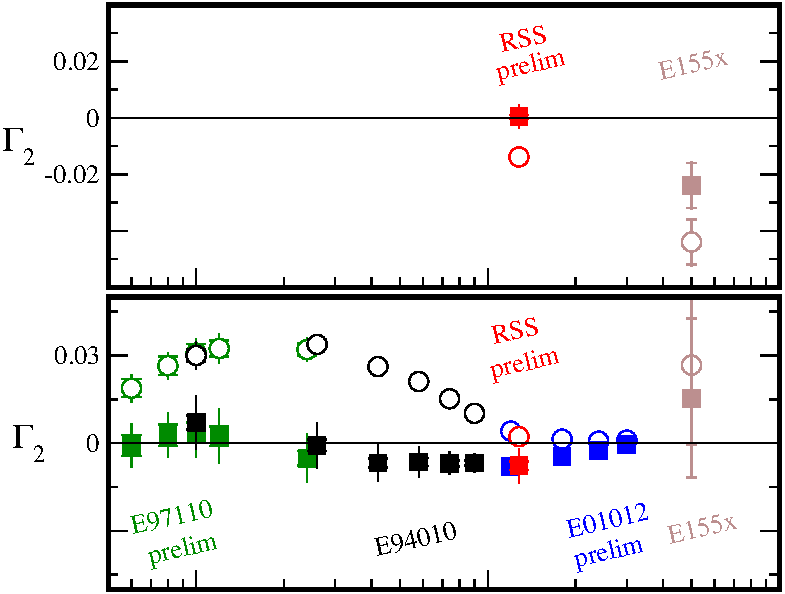
\includegraphics[width=0.75\textwidth]{figs/BC_all.pdf}}
    \put(3.5,0.1){\makebox{$Q^2$ (GeV${}^2$)}}
    \put(1.7,0.5){\makebox{\small 0.1}}
    \put(4.6,0.5){\makebox{\small 1}}
    \put(7.3,0.5){\makebox{\small 10}}
    \put(1.2,1.0){\colorbox{white}{\makebox(5.8,0.7){\textcolor{white}{a}}}}
    \put(4.5,2.8){\colorbox{white}{\makebox(1.5,0.7){\textcolor{white}{a}}}}
    \put(4.5,5.5){\colorbox{white}{\makebox(2.5,0.7){\textcolor{white}{a}}}}
  \end{picture}
  \caption[The verification of the BC sum rule.]{The verification of the BC sum rule from JLab Hall C experiment RSS (red) and Hall A experiments E94-010 \cite{Amarian2004a} (black), E97-110 (green) and E01-012 (blue), together with SLAC E155x \cite{Anthony2003} (brown). The open circles are the measured values and the solid squares are the total moments including the elastic and estimated contributions from high energy region. The data from experiments RSS and E97-110 are still preliminary. Plot reproduced from \cite{Chen2010}. \label{C4S3F1}}
\end{figure}

On the other hand, the proton BC integral deviated from zero by three standard deviations in SLAC E155x \cite{Abe1998}. E155x covered the $x$ range from 0.02 to 0.8 and its $Q^2$ coverage $0.8-8.2$ GeV${}^2$ was averaged to 5 GeV${}^2$. JLab experiment RSS also measured the BC integral for proton which covered $W<1.910$ MeV at $Q^2\approx1.3$ GeV${}^2$. The preliminary result agrees with the BC sum rule prediction within the experimental error. The experimental results for verification of the BC sum rule are summarized in \Cref{C4S3F1}.

\section{Proton Hyperfine Structure}
\label{C4S4}

The hydrogen hyperfine splitting has been measured to a relative accuracy of $10^{-13}$ according to the discussion in Ref. \cite{Nazaryan2006}:
\begin{equation} \label{C4S4E1}
\Delta E = 1420.405 751 766 7(9) \text{MHz}.
\end{equation}
This value could be calculate in QED. $\Delta E$ can be expressed in terms of the so-called Fermi energy $E_F$ which is the leading order contribution to the ground state hyperfine splitting as $\Delta E = (1+\delta)E_F$, where the correction $\delta$ is given by:
\begin{equation} \label{C4S4E2}
\delta = 1+(\delta_{\mathrm{QED}}+\delta_R+\delta_{\mathrm{small}})+\Delta_S.
\end{equation}
Here the $\delta_{\mathrm{QED}}$ represents the QED radiative correction which has been calculated to very high accuracy. The $\delta_R$ accounts the recoil effects and the $\delta_{\mathrm{small}}$ term contains all other small corrections such as the weak interaction correction.

The $\Delta_S$ term in \cref{C4S4E2} represents the proton structure correction which has the largest uncertainty. $\Delta_S$ is conventionally split into two terms:
\begin{equation} \label{C4S4E3}
\Delta_S = \Delta_Z+\Delta_{\mathrm{pol}},
\end{equation}
where $\Delta_Z$ can be determined from elastic scattering \cite{GEP} and $\Delta_{\mathrm{pol}}$ contains the contributions from excited proton \cite{Iddings1965,Faustov2002}:
\begin{equation} \label{C4S4E4}
\Delta_{\text{pol}} = \frac{\alpha m_e}{\pi g_pm_p}(\Delta_1+\Delta_2),
\end{equation}
where $\Delta_1$ involves the Pauli form factor and the $g_1$ structure function, and $\Delta_2$ only depends on the $g_2$ structure function:
\begin{equation} \label{C4S4E5}
\Delta_2 = -24m_p^2\int_0^{\infty}\frac{\dd{Q}^2}{Q^4}B_2(Q^2),
\end{equation}
where
\begin{equation} \label{C4S4E6}
B_2(Q^2) = \int_0^{x_{\mathrm{th}}}\dd{x}\beta_2(\tau)g_2(x,Q^2).
\end{equation}
and
\begin{equation} \label{C4S4E7}
\beta_2(\tau) = 1+2\tau-2\sqrt{\tau(\tau+1)},
\end{equation}
with $\tau=\nu^2/Q^2$ and $x_{\mathrm{th}}$ is the pion production threshold.

$\Delta_1$ could be determined with data but to evaluate $\Delta_2$ physicists still heavily rely on models since proton $g_2$ data are still lacking. The $Q^2$ weighting in \cref{C4S4E5} indicates that $\Delta_2$ is dominated by the contribution at low $Q^2$ \cite{Nazaryan2006}. Thus, precision data of proton $g_2$ at low $Q^2$ is needed to evaluate $\Delta_2$.

%%%%%%%%%%%%%%%%%%%%%%%%%%%%%%%%%%%%%%%%%%%%%%%%%%%%%%%%%%%%%%%%%%%%%%
% -*-latex-*-
